\documentclass{article}

\title{IC internals: XNet protocol}
\subtitle{A deep dive into the protocol that IC subnets communicate over.}
\date{2022-07-01}
\modified{2022-07-01}

\keyword{ic}

\begin{document}
\section{introduction}{Introduction}

This article continues the previous post on state machine replication in the Internet Computer (IC), \nameref{02-ic-state-machine-replication}.
This time, we shall examine the protocol over which independent state machines (also known as \emph{subnets}) communicate, the \emph{XNet protocol}.

\section{subnets}{Subnets}

A \emph{subnet} is a collection of nodes participating in a single instance of the \href{https://dfinity.org/howitworks/consensus}{consensus protocol}.
All the nodes in a subnet have the same state and apply the same blocks.

It might be tempting to think that nodes of a subnet are physically collocated.
However, the opposite is usually true: subnet nodes are often geographically distributed across independent data centers\sidenote{sn-dc-nodes}{
  There are still good reasons to assign multiple nodes in a data center to the same subnet, such as increasing query call capacity and speeding up recovery in case of a replica restart.
}.
The goal is to improve availability: a disaster in a single data center cannot take down the entire subnet.
The \emph{registry} canister maintains the assignment of nodes to physical machines, and the \href{https://dfinity.org/howitworks/network-nervous-system-nns}{Network Nervous System} governs all the changes to the registry.

Nodes from different subnets can live in the same data center.
This setup might be counter-intuitive: nodes from different subnets might sometimes have better network connectivity than nodes in the same subnet.

\begin{figure}[grayscale-diagram]
  \marginnote{mn-subnets}{
    Two three-node subnets located in three data centers.
    Solid lines represent peer-to-peer communication within a subnet; dotted lines — cross-subnet communication.
    Not all XNet connections are present in the picture.
  }
  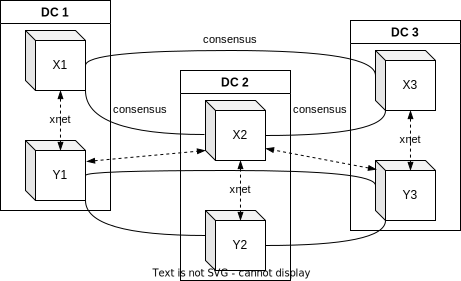
\includegraphics{/images/08-subnets.svg}
\end{figure}

XNet protocol is not limited to the same-datacenter communication; any node from one subnet can talk to any other node from another subnet.
However, the replica prefers contacting close\sidenote{mn-proximity}{
  The replica uses network latency as the proximity measure.
  It randomly contacts nodes from other subnets, assigning higher weights to nodes with lower latency.
} peers to reduce the message delivery latency.

\section{message-streams}{Message streams}

Messages start their journey in the output queues of canisters hosted on the source subnet.
The subnet sorts these messages based on the destination subnet and interleaves them into flat message streams (one stream per destination subnet).
Each message in the stream gets a unique monotonically increasing index.

\begin{figure}[grayscale-diagram]
  \marginnote{mn-message-streams}{
    The flow of messages within a subnet.
    Canisters push messages into their output queues; the stream builder picks up these messages and constructs a flat outgoing message stream for each subnet.
  }
  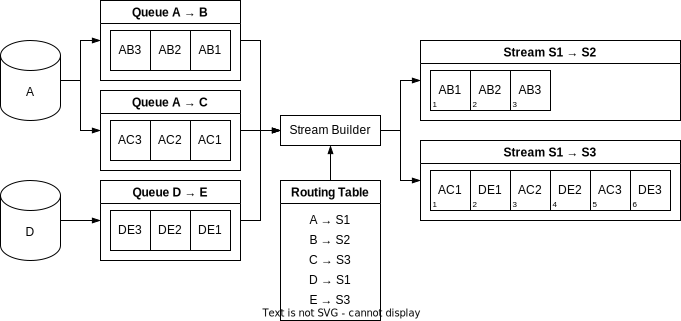
\includegraphics{/images/08-message-streams.svg}
\end{figure}

The component merging the queues (aptly called \emph{stream builder}) should satisfy a few constraints:
\begin{itemize}
  \item
  \emph{Determinism}.
  All nodes in the subnet must agree on the exact contents of the stream.
  To do its job, the stream builder needs the mapping from canister identifiers to subnet identifiers, the \emph{routing table}.
  The routing table comes from the registry and changes over time.
  To ensure determinism, each block pins the registry version that the state machine is using for message processing.
  \item
  \emph{Ordering}.
  If canister \math{A} sends two requests to canister \math{B}, \math{R\sub{1}}, and \math{R\sub{2}}, then \math{R\sub{1}} should appear before \math{R\sub{2}} in the stream.
  \item
  \emph{Fairness.}
  We do not want messages from a single chatty canister to dominate the stream.
  The stream builder tries to interleave messages so that each canister has the same bandwidth.
\end{itemize}

When a node from subnet \math{X} decides to get new messages from subnet \math{Y}, it picks a node from \math{Y} (the registry stores the entire network topology) and calls \math{Y}'s XNet endpoint with the index of the first unseen message and the number of messages to fetch.

\section{block-payloads}{Block payloads}

The job of the consensus protocol is to aggregate messages from the outside world and pack them into a neat block.
Consensus includes several types of messages into blocks, such as user ingress messages, Bitcoin transactions (for subnets with enabled Bitcoin integration), and inter-canister messages from other subnets.
We call messages paired with the data required for their validation a \emph{payload}.
We call components that pull payloads from the network \emph{payload builders}.

\begin{figure}[grayscale-diagram]
  \marginnote{mn-payloads}{The consensus algorithm aggregates messages from the outside world into blocks.}
  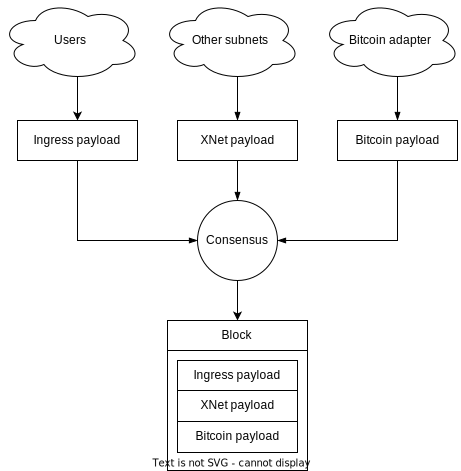
\includegraphics{/images/08-block-payloads.svg}
\end{figure}

XNet payload builder pulls messages from nodes assigned to other subnets using a simple HTTP protocol.
\emph{XNet endpoint} is a component that serves messages destined for other subnets over secure TLS connections, accepting connections only from other nodes\sidenote{sn-xnet-tls}{This measure does not imply privacy because malicious nodes can access the data; but ensures that network providers cannot read the messages.}.
XNet endpoint fetches the complete list of nodes, their subnet assignment, IP addresses, and public keys (required to establish a TLS connection) from the registry.

\begin{figure}[grayscale-diagram]
  \marginnote{mn-endpoint}{
    The data flow in the XNet protocol.
    Subnet \math{Y} produces a signed stream of messages for subnet X and exposes this stream via an HTTP endpoint.
    Subnet \math{X} pulls messages from one of the nodes on subnet Y.
  }
  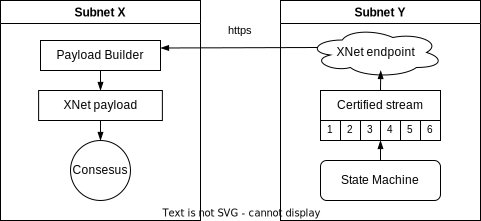
\includegraphics{/images/08-xnet-endpoint.svg}
\end{figure}

\section{garbage-collection}{Garbage collection}

We now know how one subnet accumulates messages destined for another subnet.
This knowledge begs another question: how do replicas remove messages that the destination subnet has already consumed?
We need a feedback mechanism allowing the consumer subnet to tell the producer subnet that it does not need some stream prefix anymore.
We call this mechanism \emph{signals}.

Signals are a part of the XNet payload specifying the prefix of the \emph{reverse} stream that the sending subnet can drop.
When a node from subnet \math{X} fetches XNet payload from a node from subnet \math{Y}, in addition to actual messages, the \math{Y} node includes the \emph{stream header}.
The stream header describes the state of the \math{X ↔ Y} communication:

\begin{itemize}
  \item
    The full range of message indices in the forward stream \math{X → Y}.
  \item
    The signals for the \emph{reverse} stream (\math{Y → X}): for each message index in the reverse stream, \math{Y} tells whether \math{X} can garbage collect the message (an \textsc{ack} signal) or should reroute the message (a \textsc{reject} signal).
    A \textsc{reject} signal indicates that the destination canister moved, so \math{X} should route the message into another stream.
\end{itemize}

Signals solve the issue of collecting obsolete messages, but they introduce another problem: now we also need to garbage-collect signals!
Luckily, we already have all the information we need: we keep signals only for messages that are still present in the reverse stream.
Once we notice (by looking at the range of message indices) that the remote subnet dropped messages from its stream, we can remove the corresponding signals from our header.

From my experience, the interplay of message indices and signals is notoriously hard to grasp, so let us look at an example.
The diagram below depicts two subnets, \math{X} and \math{Y}, caught in the middle of communication.
Subnet \math{X} gets a prefix of \math{Y}'s stream and the header, allowing \math{X} to induct new messages and garbage-collect its messages and signals.
\math{X} also publishes signals for the newly received messages and updates its indices accordingly so that \math{Y} could garbage-collect its messages and signals in the next round of communication.

\begin{figure}[grayscale-diagram]
  \marginnote{mn-signals}{
    Two subnets, \math{X} and \math{Y}, communicating over the XNet protocol.
    In previous communications, subnet \math{Y} consumed messages \math{\[0,10)} from \math{X}'s stream and has recently received messages \math{10} and \math{11}.
    Now, subnet \math{X} receives a prefix of \math{Y}'s stream and the matching header and removes messages \math{10} and \math{11} from its stream because \math{Y} will not need them anymore.
    \math{X} also includes signals for the newly received messages into the \math{X → Y} stream header and removes an obsolete signal for message \math{Y\sub{1}} it consumed before.
  }
  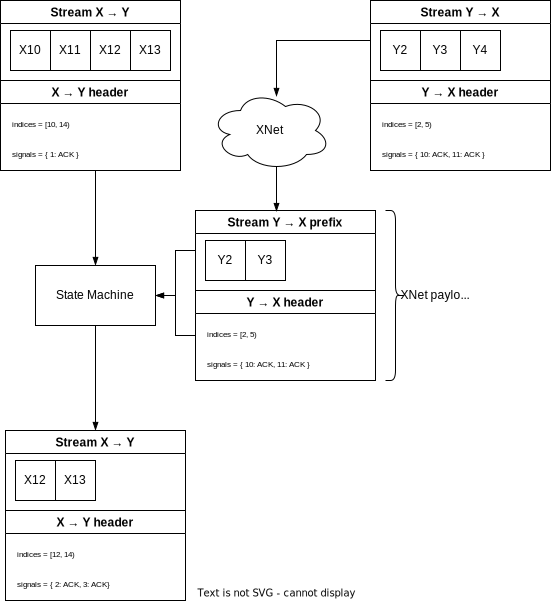
\includegraphics{/images/08-signals.svg}
\end{figure}

Signals and stream messages are like snakes eating each other's tails on the \href{https://theneverendingstory.fandom.com/wiki/Auryn}{Auryn}: the sender drops messages when it sees signals, and the receiver drops signals when it sees stream bounds advancing.

\section{stream-certification}{Stream certification}

Since no two nodes in the network can blindly trust each other, we need a mechanism to validate the contents of XNet payloads.
More specifically, we want proof that the stream prefix in the payload is the same on all honest nodes in the subnet that produced the stream.
In the previous article, we have seen how nodes use threshold signatures on \href{/posts/02-ic-state-machine-replication.html#state-trees}{state trees} as authenticity proofs for call replies.
The XNet protocol relies on the same trick: nodes include streams destined for other subnets into their state trees and use threshold signatures as proofs of authenticity for nodes from other subnets.

\begin{figure}[grayscale-diagram]
  \marginnote{mn-certification}{
    The encoding of subnet message streams in the \href{/posts/02-ic-state-machine-replication.html#state-trees}{state tree}.
  }
  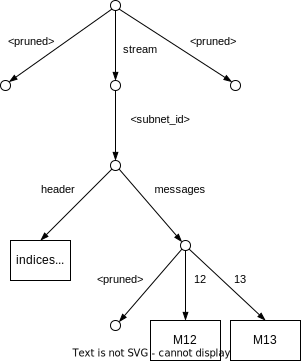
\includegraphics{/images/08-certification.svg}
\end{figure}

Conceptually, a node requesting messages from a subnet is not different from a client requesting a response.
This similarity allows us to use the same\sidenote{sn-same-auth}{
  Currently, there is a minor difference in how we represent certificates in the XNet protocol and the \href{https://internetcomputer.org/docs/current/references/ic-interface-spec/#_certificate}{IC HTTP} interface.
  The HTTP interface certificates combine the data and the hashes required to check the authenticity in a single data structure, the \emph{hash tree}.
  The XNet protocol separates the raw message data and the hashes (called the \emph{witness}) into separate data structures.
  The reason for that distinction is purely historical.
  We implemented the XNet protocol significantly earlier than the response authentication, so we could not benefit from \href{https://www.joachim-breitner.de/blog}{Joachim Breitner's} brilliance.
  Joachim took the XNet authentication scheme as the starting point and simplified it for the IC Interface Specification.
} authentication mechanism in both cases.

The tree structure of the certificate comes in handy for buffering messages on the receiver: the receiver can maintain a slightly larger pool of messages than a single block can fit, asynchronously fetching new messages and appending them to the pool, merging the certificates appropriately.
This optimization allows us to use the subnet's narrow XNet channel more efficiently and improve fairness when we include messages from multiple subnets into a single block.

\section{limitations}{Limitations}

The XNet protocol is a marvelous feat of engineering, but it has a few inherent limitations:
\begin{itemize}
  \item
    All XNet messages have to go through consensus blocks.
    This constraint bounds the theoretical throughput of the protocol by the block rate and size.
    For example, if a subnet produces one block every second and the block size is 2MiB, the XNet throughput on this subnet can be at most 2MiB/sec.
  \item
    Delivering a message requires two rounds of consensus (one round on the sender, one round on the receiver).
    This constraint bounds the latency of the protocol by the block rate.
    If both the receiving and the sending subnet need a second to produce a block, a request will need at least two seconds to reach the destination.
    Delivering the response will need another two rounds, so the call round-trip time is at least four seconds.
\end{itemize}

\section{references}{Code references}

A few pointers to the code implementing designs from this article:
\begin{itemize}
  \item The \href{https://github.com/dfinity/ic/blob/226faa85b945aabf0fc22a18b4c2e1b9f0f4c8ee/rs/registry/routing_table/src/lib.rs#L213}{routing table}.
  \item The \href{https://github.com/dfinity/ic/blob/226faa85b945aabf0fc22a18b4c2e1b9f0f4c8ee/rs/messaging/src/routing/stream_builder.rs#L237}{stream builder}.
  \item The \href{https://github.com/dfinity/ic/blob/226faa85b945aabf0fc22a18b4c2e1b9f0f4c8ee/rs/xnet/payload_builder/src/lib.rs#L665}{payload builder} and the \href{https://github.com/dfinity/ic/blob/226faa85b945aabf0fc22a18b4c2e1b9f0f4c8ee/rs/xnet/payload_builder/src/certified_slice_pool.rs#L1042}{XNet message buffer}.
  \item The \href{https://github.com/dfinity/ic/blob/226faa85b945aabf0fc22a18b4c2e1b9f0f4c8ee/rs/xnet/endpoint/src/lib.rs#L93}{XNet endpoint} and the \href{https://github.com/dfinity/ic/blob/226faa85b945aabf0fc22a18b4c2e1b9f0f4c8ee/rs/xnet/payload_builder/src/proximity.rs#L118}{node proximity metric} computation.
  \item The \href{https://github.com/dfinity/ic/blob/226faa85b945aabf0fc22a18b4c2e1b9f0f4c8ee/rs/messaging/src/routing/stream_handler.rs#L557}{induction of messages} into the state machine state.
  \item The garbage collection of \href{https://github.com/dfinity/ic/blob/226faa85b945aabf0fc22a18b4c2e1b9f0f4c8ee/rs/messaging/src/routing/stream_handler.rs#L391-L426}{messages} and \href{https://github.com/dfinity/ic/blob/226faa85b945aabf0fc22a18b4c2e1b9f0f4c8ee/rs/messaging/src/routing/stream_handler.rs#L428-L465}{signals}.
  \item The \href{https://github.com/dfinity/ic/blob/226faa85b945aabf0fc22a18b4c2e1b9f0f4c8ee/rs/canonical_state/src/lazy_tree/conversion.rs#L254-L284}{mapping of streams} to the tree structure, \href{https://github.com/dfinity/ic/blob/226faa85b945aabf0fc22a18b4c2e1b9f0f4c8ee/rs/state_manager/src/stream_encoding.rs#L40}{tree encoding}, and \href{https://github.com/dfinity/ic/blob/226faa85b945aabf0fc22a18b4c2e1b9f0f4c8ee/rs/state_manager/src/lib.rs#L2912-L2972}{validation}.
\end{itemize}

\section{credits}{Credits}

Finally, I shall give due credit to people who played an essential role in the protocol development.
\begin{itemize}
\item
  \href{https://www.linkedin.com/in/allen-clement-b73a4652/}{Allen Clement} is the mastermind behind most of the features of the XNet protocol.
\item
  \href{https://www.linkedin.com/in/david-derler-08630495/}{David Derler} refined many of Allen's ideas and wrote a formal mathematical specification for the protocol.
\item
  \href{https://www.linkedin.com/in/alin-sinpalean-8451b8139/}{Alin Sinpalean} implemented the protocol in the \href{https://github.com/dfinity/ic/tree/3fe4137c86ab0521c39089954c03d7fb29e2c3d2/rs/xnet}{IC replica} and developed many optimizations.
\end{itemize}

My main contributions are stream certification and TLS integration.
\end{document}
